% A schematic diagram showing the model architecture.
% In each of the encoder, decoder and bottom blocks the feature map is transformed with two successive 
% 3x3x3 convolutions followed by a ReLU activation function.
% Blocks in the contracting path are downsampled with a 2x2x2 max-pooling operation;
% blocks in the expanding bath are upsampled with a 2x2x2 upsampling operation. (check this)
% An attention mechanism brings information from coarser scales in to the skip connection.
% The feature map from deeper in the network acts as the attention gating signal.
% The gated feature map from the encoder path is concatenated with upsampled feature map from
% the deeper layer along the channel dimension.
% A convolution along the channel dimension gives the feature map that is fed to each decoder block.

\documentclass{standalone}
\usepackage{tikz}
\usetikzlibrary{shapes.geometric, arrows.meta, positioning}

\tikzstyle{block} = [rectangle, draw, text centered, minimum height=1cm, minimum width=3cm, text width=4cm, rotate=90]
\tikzstyle{arrow} = [thick,->,>=stealth]
\tikzstyle{skip} = [thick, dashed,->,>=stealth]
\tikzstyle{attention} = [circle, draw, text centered, minimum height=1cm, minimum width=2em]

\begin{document}
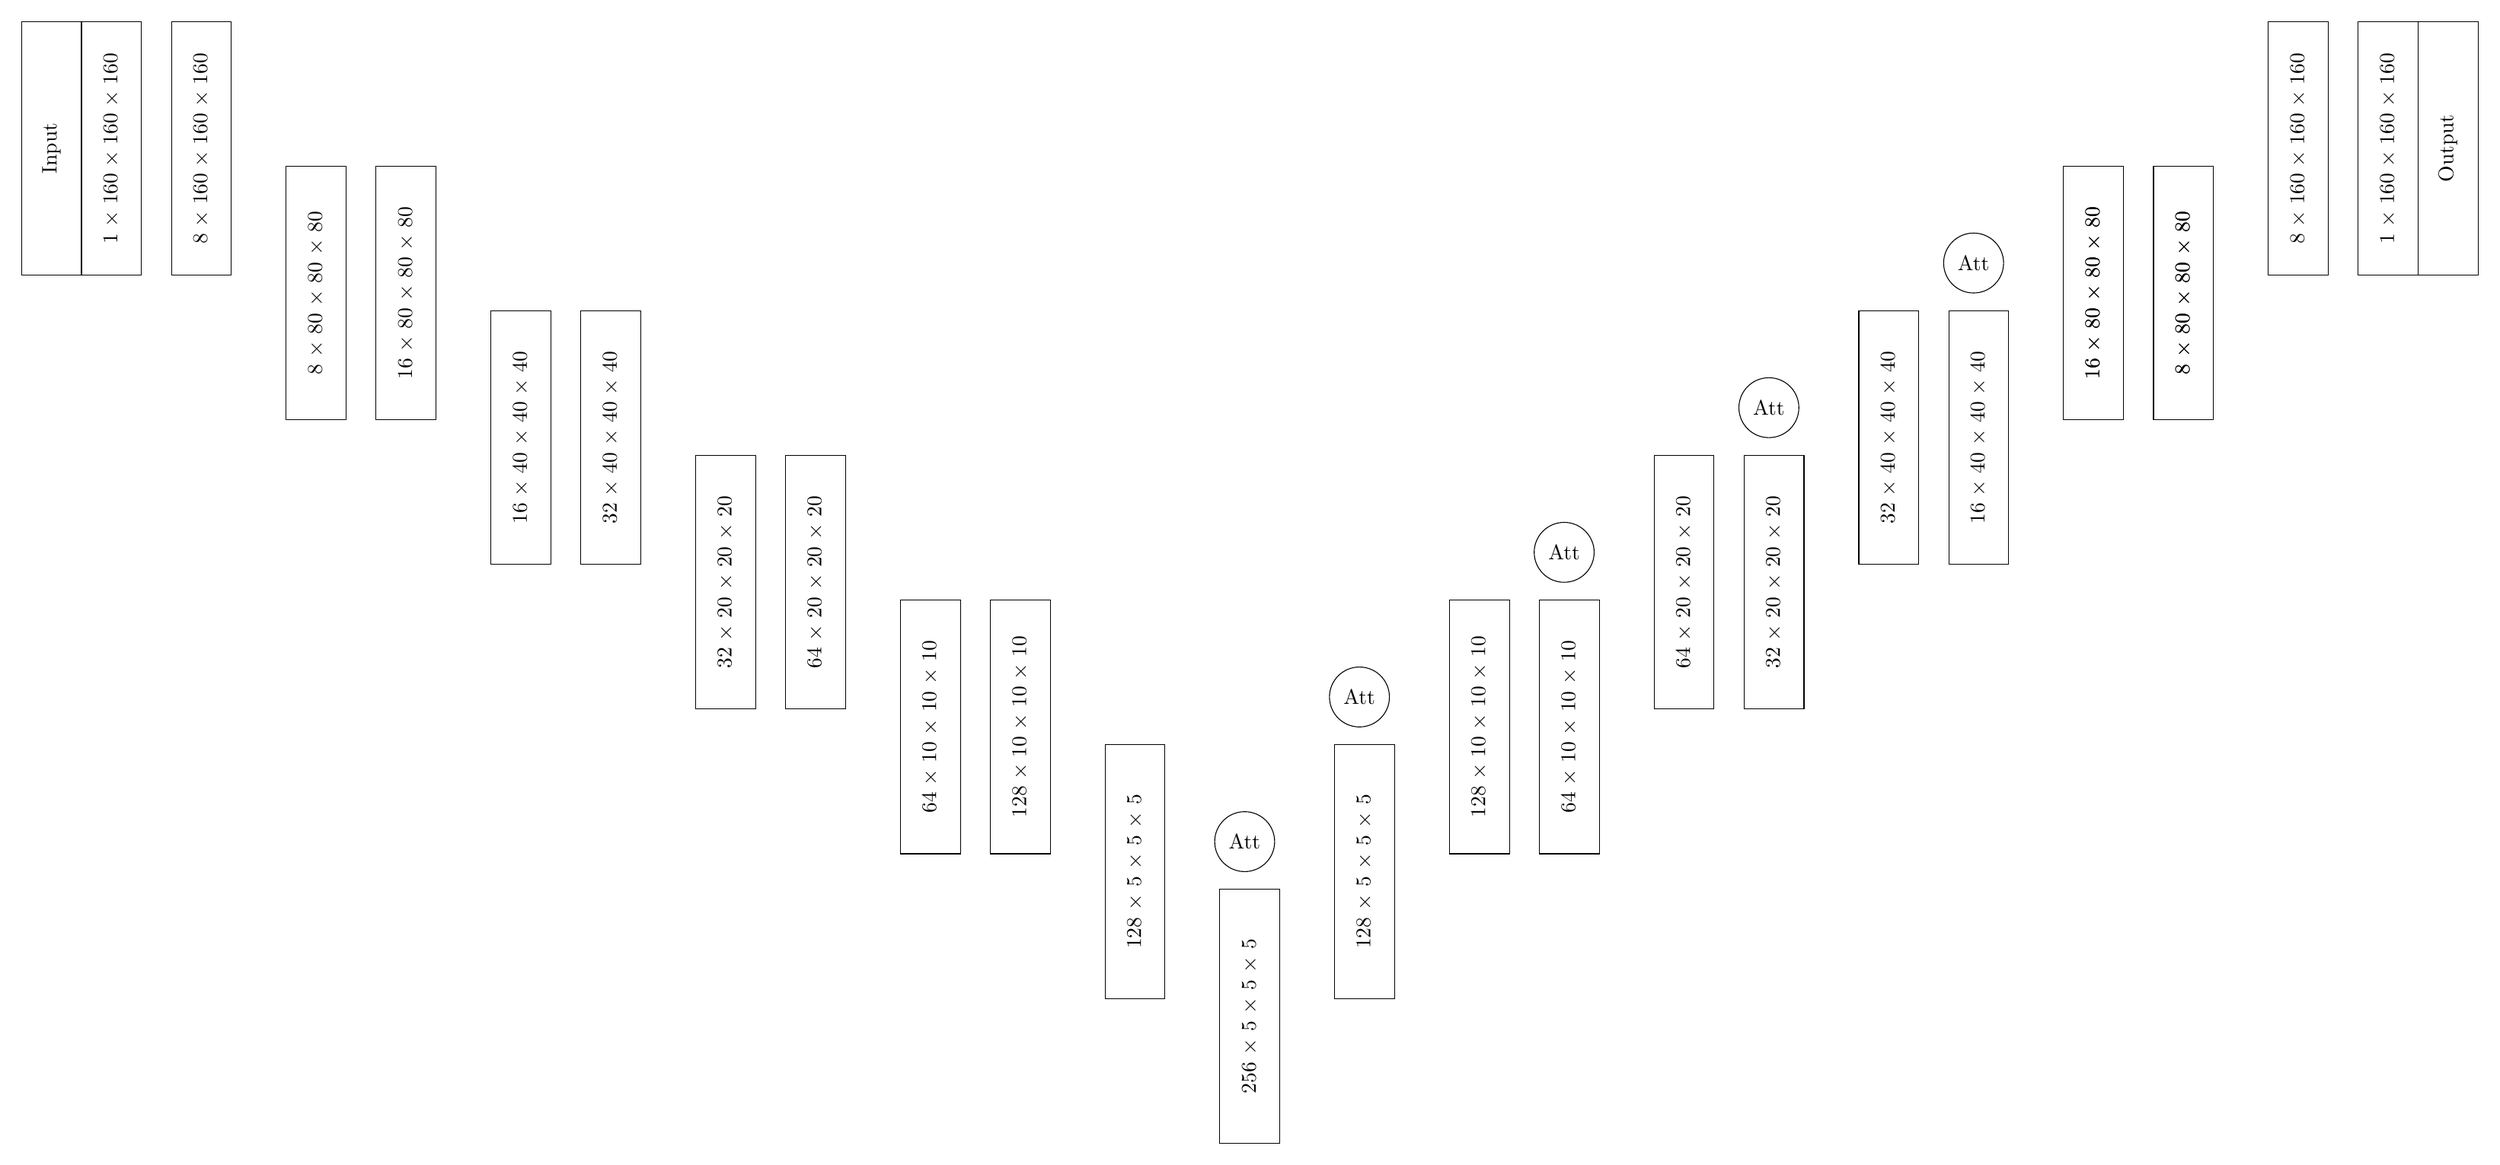
\begin{tikzpicture}[node distance=2cm]

    % Input
    \node (input_label) [block] {Input};
    \node (input) [block, below of=input_label, yshift=1cm]{$1\times160\times160\times160$};

    % Contracting path
    \node (head) [block, below of=input, yshift=0.5cm] {$8\times160\times160\times160$};

    \node (enc1) [block, below left of=head, yshift=-0.5cm, xshift=-1cm]{$8\times80\times80\times80$};
    \node (conv1) [block, below of=enc1, yshift=0.5cm]{$16\times80\times80\times80$};

    \node (enc2) [block, below left of=conv1, yshift=-0.5cm, xshift=-1cm]{$16\times40\times40\times40$};
    \node (conv2) [block, below of=enc2, yshift=0.5cm]{$32\times40\times40\times40$};

    \node (enc3) [block, below left of=conv2, yshift=-0.5cm, xshift=-1cm]{$32\times20\times20\times20$};
    \node (conv3) [block, below of=enc3, yshift=0.5cm]{$64\times20\times20\times20$};

    \node (enc4) [block, below left of=conv3, yshift=-0.5cm, xshift=-1cm]{$64\times10\times10\times10$};
    \node (conv4) [block, below of=enc4, yshift=0.5cm]{$128\times10\times10\times10$};

    \node (enc5) [block, below left of=conv4, yshift=-0.5cm, xshift=-1cm]{$128\times5\times5\times5$};

    % Bottom layer
    \node (bottom) [block, below left of=enc5, yshift=-0.5cm, xshift=-1cm]{$256\times5\times5\times5$};

    % Expanding Path
    \node (conv6) [block, below right of=bottom, yshift=-0.5cm, xshift=1cm] {$128\times5\times5\times5$};

    \node (dec4) [block, below right of=conv6, yshift=-0.5cm, xshift=1cm]{$128\times10\times10\times10$};
    \node (conv7) [block, below of=dec4, yshift=0.5cm] {$64\times10\times10\times10$};

    \node (dec3) [block, below right of=conv7, yshift=-0.5cm, xshift=1cm]{$64\times20\times20\times20$};
    \node (conv8) [block, below of=dec3, yshift=0.5cm] {$32\times20\times20\times20$};

    \node (dec2) [block, below right of=conv8, yshift=-0.5cm, xshift=1cm]{$32\times40\times40\times40$};
    \node (conv9) [block, below of=dec2, yshift=0.5cm] {$16\times40\times40\times40$};

    \node (dec1) [block, below right of=conv9, yshift=-0.5cm, xshift=1cm]{$16\times80\times80\times80$};
    \node (conv10) [block, below of=dec1, yshift=0.5cm] {$8\times80\times80\times80$};

    \node (dec1) [block, below right of=conv9, yshift=-0.5cm, xshift=1cm]{$16\times80\times80\times80$};
    \node (conv10) [block, below of=dec1, yshift=0.5cm] {$8\times80\times80\times80$};

    \node (dec0) [block, below right of=conv10, yshift=-0.5cm, xshift=1cm]{$8\times160\times160\times160$};

    % Output
    \node (output) [block, below of=dec0, yshift=0.5cm] {$1\times160\times160\times160$};
    \node (output_label) [block, below of=output, yshift=1cm]{Output};

    % % Attention Mechanisms
    \node (att5) [attention, above right of=bottom, xshift=-1.5cm, yshift=1.5cm] {Att};
    \node (att4) [attention, above right of=conv6, xshift=-1.5cm, yshift=1.5cm] {Att};
    \node (att3) [attention, above right of=conv7, xshift=-1.5cm, yshift=1.5cm] {Att};
    \node (att2) [attention, above right of=conv8, xshift=-1.5cm, yshift=1.5cm] {Att};
    \node (att1) [attention, above right of=conv9, xshift=-1.5cm, yshift=1.5cm] {Att};

    % ==== Arrows
    % Contracting
    % \draw [arrow] (input) -- (head);
    % \draw [arrow] (head_size) -- (enc1_size);
    % \draw [arrow] (enc1_size) -- (enc2_size);
    % \draw [arrow] (enc2_size) -- (enc3_size);
    % \draw [arrow] (enc3_size) -- (enc4_size);
    % \draw [arrow] (enc4_size) -- (enc5_size);
    % \draw [arrow] (enc5_size) -- (bottom);

    % % Expanding
    % \draw [arrow] (bottom) -- (dec5);
    % \draw [arrow] (dec5) -- (dec4);
    % \draw [arrow] (dec4) -- (dec3);
    % \draw [arrow] (dec3) -- (dec2);
    % \draw [arrow] (dec2) -- (dec1);
    % \draw [arrow] (dec1) -- (reduce);
    % \draw [arrow] (reduce) -- (output);

    % % Attention
    % \draw [skip] (bottom) -- (att5);
    % \draw [skip] (dec5) -- (att4);
    % \draw [skip] (dec4) -- (att3);
    % \draw [skip] (dec3) -- (att2);
    % \draw [skip] (dec2) -- (att1);

    % % Skip Connections
    % \draw [skip] (enc5) -- (att5);
    % \draw [skip] (att5) -- (dec5);
    % \draw [skip] (enc4) -- (att4);
    % \draw [skip] (att4) -- (dec4);
    % \draw [skip] (enc3) -- (att3);
    % \draw [skip] (att3) -- (dec3);
    % \draw [skip] (enc2) -- (att2);
    % \draw [skip] (att2) -- (dec2);
    % \draw [skip] (enc1) -- (att1);
    % \draw [skip] (att1) -- (dec1);

\end{tikzpicture}
\end{document}
